\documentclass[notheorems, aspectratio=169]{beamer}
\usepackage{style}
\usepackage{cite}
\usepackage{tikz}
\usepackage{graphicx}
\usepackage{tcolorbox}

% Change the color theme in style.tex

% Change the frame numbering and box numbering
% \addtocounter{framenumber}{13}
\newcommand{\numchap}{1}

% Chapter name
\newcommand{\namechap}{AoII in Scheduling}

\setbeameroption{hide notes} % Only slides
%\setbeameroption{show only notes} % Only notes
%\setbeameroption{show notes on second screen=right} % Both
%\setbeamertemplate{note page}{\pagecolor{yellow!5}\insertnote}

% Numbered reference item
\setbeamertemplate{bibliography item}{\insertbiblabel}

% Theme Color
\setbeamercolor{background canvas}{bg=MyBlack}
\setbeamercolor{normal text}{fg=MyWhite2,bg=MyBlack}

%Table of Content Formatting
\setbeamertemplate{section in toc}{\inserttocsection}
\setbeamerfont{section in toc}{size=\LARGE}

%Title page information
\title{Minimizing Age of Incorrect Information\\[-12pt] for Unreliable Channel with Power Constraint}
\author{Yutao Chen and Anthony Ephremides}
\institute{Department of Electrical and Computer Engineering\\
			   University of Maryland, College Park}
\date{GlobeCom2021, December 2021}
% logo(s)
\logo{

\includegraphics[height=0.1\paperheight]{Figures/umd.png}
\hspace{5.5cm}

\includegraphics[height=0.1\paperheight]{Figures/ieee-globecom.png}
}

\begin{document}
% Front Page
\begin{frame}[plain, noframenumbering]
  \titlepage
\end{frame}

\begin{frame}[plain, noframenumbering]
\begin{center}
\blue{\textbf{\Large Scheduling to Minimize Age of Incorrect Information\\
\vspace{1em}
with Imperfect Channel State Information}}
\end{center}
\end{frame}

\logo{}  % Remove LOGO in other pages. Bad solution. Need fix.

\section{SECTION 1}

\begin{frame}[plain, noframenumbering]
\begin{center}
\textbf{\tableofcontents[currentsection]}
\end{center}
\end{frame}

\begin{frame}{Frame Title}{Frame Subtitle}
\newparagraph{Equation}
\begin{equation}
arg\min_{\phi \in \Phi}\ {\lim_{T\to\infty} \frac{1}{T} \mathbb{E}\left[\sum_{t=0}^{T-1} s^{\phi}(t) \ | \ \phi,(d(0),s(0))\right]}
\end{equation}
\note[item]{Note that this slide is boring.}
\sep $\Phi$ is the collection of all feasible series of actions \sep $s^{\phi}(t)$ is the penalty paid at time $t$ when the \primary{transmitter acted} following the series of actions $\phi$ \sep $(d(0),s(0))$ are the initial values of the difference and the penalty respectively
\bigbreak
\newparagraph{Normal text}\\
Some text\cite{b1}
\end{frame}

\section{SECTION 2}

\begin{frame}[plain, noframenumbering]
\begin{center}
\textbf{\tableofcontents[currentsection]}
\end{center}
\end{frame}

\begin{frame}{Frame Title}
\newparagraph{Columns}
\begin{columns}
\begin{column}{0.5\textwidth}
\begin{itemize}
\item The command creates the frame environment, see full example to the right.
\begin{itemize}
\item Options are for setting frame labels or template specific frame types -- see next slide and the examples section
\end{itemize}
\item Examine the main.tex file and Beamer class for more \LaTeX\ code examples
\end{itemize}
\end{column}
\begin{column}{0.5\textwidth}
\begin{itemize}
\item The command creates the frame environment, see full example to the right.
\item Options are for setting \primary{frame labels or template specific} frame types -- see next slide and \cite{b2} the examples section 
\item Examine the main.tex file and Beamer class for more \LaTeX\ code examples
\end{itemize}
\end{column}
\end{columns}
\vspace{1em}

\newparagraph{Enumerate}
\begin{enumerate}
\item item 1
\begin{enumerate}
\item text
\begin{enumerate}
\item Text2
\end{enumerate}
\end{enumerate}
\item item 2
\end{enumerate}
\end{frame}

\begin{frame}{Frame Title}
\newparagraph{Figure}
\begin{columns}
\begin{column}{0.5\textwidth}

\begin{center}
\begin{figures}
    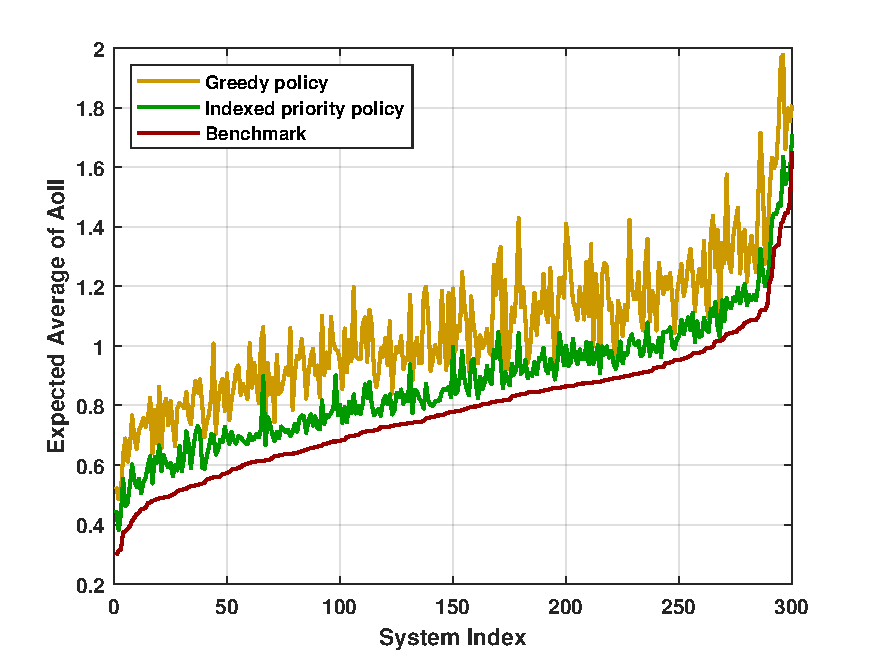
\includegraphics[width=\linewidth]{Figures/Random.pdf}
\end{figures}
\blue{Figure:} Random system settings
\end{center}

\end{column}
\begin{column}{0.5\textwidth}

\begin{center}
\begin{figures}
    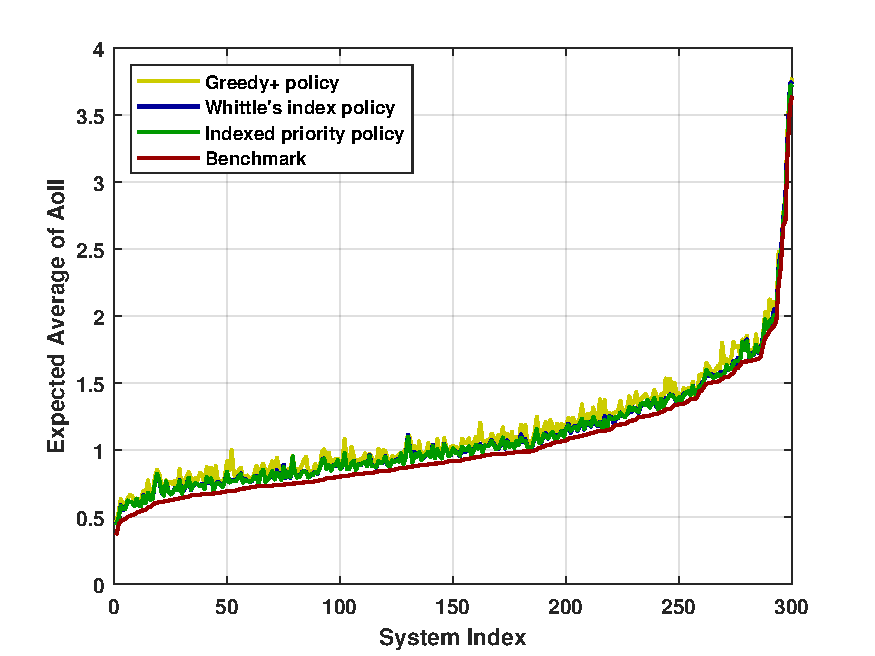
\includegraphics[width=\linewidth]{Figures/Random_Whittle.pdf}
\end{figures}
\blue{Figure:} Random system settings with Whittle
\end{center}

\end{column}
\end{columns}

\end{frame}

\begin{frame}{Frame Title}
\newparagraph{Table}
\begin{table}[htbp]
\renewcommand{\arraystretch}{1.2}
\centering
\caption{Optimal thresholds for different $p$}
\begin{tabular}{c|c|c|c|c|c|c|c}
    \hline
    & Mixing Coef. & $n_1$ & $n_2$ & $n_3$ & $n_4$ & $n_5$ & $n_6$\\
    \hline
    \hline
    $p=0.1$ & $\mu=0.7176$ & 15 & 6/7 & 1 & 1 & 1 & 1\\ 
    \hline
    $p=0.2$ & $\mu=0.0331$ & 37 & 16 & 8/9 & 1 & 1 & 1\\ 
    \hline
    $p=0.3$ & $\mu=0.1178$ & 69 & 25/26 & 15 & 1 & 1 & 1\\ 
    \hline
\end{tabular}
\end{table}
\end{frame}

\section{SECTION 3}

\begin{frame}[plain, noframenumbering]
\begin{center}
\textbf{\tableofcontents[currentsection]}
\end{center}
\end{frame}

\begin{frame}{Frame Title}
\newparagraph{Blocks}
\begin{theorem}[label = {theo-test1}]{Optimal Policy}
Theorem
\end{theorem}
\begin{lemma}[label = {lem-test1}]{Monotone}
lemma
\end{lemma}
\pause
\begin{corollary}[label = {cor-test1}]{Consequences}
corollary
\end{corollary}
\begin{proposition}[label = {prop-test1}]{Structural Property}
proposition
\end{proposition}
\end{frame}

\begin{frame}{Frame Title}
\newparagraph{More Blocks}
\begin{definition}{Statistically Identical}
Definition
\end{definition}
\begin{assumption}{Perfect CSI}
assumption
\end{assumption}
\pause
\begin{remark}
Remark
\end{remark}
\begin{example}{Machine Overheating}
Example
\end{example}
\end{frame}

\begin{frame}{Frame Title}
\newparagraph{Blocks references}
According to Theorem \numchap.\ref{theo-test1}, Lemma \ref{lem-test1}, Corollary \ref{cor-test1}, and Proposition \ref{prop-test1}.

\end{frame}

\begin{frame}[plain]{Summary}
\begin{description}[Other description]
	\item[Combination] is a combination of age-based metrics framework.
    \item[Sufficiency] characterize the ”Real-time Error” metric in some systems and for some choices of penalty functions.
    \item[Semantic] communication goal is taken into account.
\end{description}

% Thank you and Info section
\vfill
\begin{columns}
\begin{column}{0.5\textwidth}
	\centering \huge
	\textcolor{MyBlue}{Thank You!}
\end{column}
\textcolor{gray!80!white}{\vrule{}}
\begin{column}{0.5\textwidth} 
	\centering \Large
	%\textcolor{MyBlue}{Yutao Chen}\\
	\textcolor{MyBlue}{cheny@umd.edu}
\end{column}
\end{columns}
\end{frame}

\begin{frame}[plain]{References}
\bibliographystyle{plain}
\bibliography{mybib}
\end{frame}

\end{document}